In this chapter we discuss the first set of four SCF algorithms that
was implemented for the LinkR application and then show how each
algorithm performed during the live user trial, how satisfied the
users were with links being recommended to them through LinkR, and the
results of offline passive experiments with the algorithms.

\subsection{Algorithms}

The CF and SCF algorithms used for the first user trial were:

\begin{enumerate}
\item{ {\bf $k$-Nearest Neighbor (KNN)}: We use the user-based approach as described in Section~\ref{sec:nn}.}
\item{{\bf Support Vector Machines (SVM)}: We use the the SVM implementation described in Section~\ref{sec:svm} using the features described in Section~\ref{sec:dataset}.}
\item{{\bf Matchbox (Mbox)}: Matchbox MF  + L2 $U$ Regularization + L2 $V$ Regularization}
\item{{\bf Social Matchbox (Soc. Mbox)}: Matchbox MF + Social Regularization + L2 Regularization}
\end{enumerate}

Social Matchbox uses the Social Regularization method to incorporate the social information of the FB data. SVM incorporates social information in the $\f_{\x,\y}$ features that it uses. Matchbox and Nearest Neighbors do not make use of any social information.

\subsection{Online Results}

The first live user trial was run from August 25 to October 13. The algorithms were randomly distributed among the 106 users who installed the LinkR application. The distribution of the algorithms to the users are show in Table~\ref{tab:Assigned1}

\begin{table}[t!]
\centering
\begin{tabular}{| l | c |}
\hline
{\bf Algorithm} & {\bf Users} \\
\hline
Social Matchbox & 26\\
Matchbox  & 26 \\
SVM & 28 \\
Nearest Neighbor & 28 \\
\hline
\end{tabular}
\caption{Number of Users Assigned per Algorithm.}
\label{tab:Assigned1}
\end{table}

Each user was recommended three links everyday and they were able to
rate the links on whether they `Liked' or `Disliked' it. Results shown
in Figure~\ref{fig:OnlineResult1} are the percentage of Like ratings
and the percentage of Dislike ratings per algorithm stacked on top of
each other with the Like ratings on top.

As shown in Figure~\ref{fig:OnlineResult1}, Social Matchbox was the
best performing algorithm in the first trial and in fact was the only
algorithm to get receive more like ratings than dislike ratings. This
would suggest that using social information does indeed provide useful
information that resulted in better link recommendations from LinkR.

\begin{figure*}[t!]
\centering
\subfigure{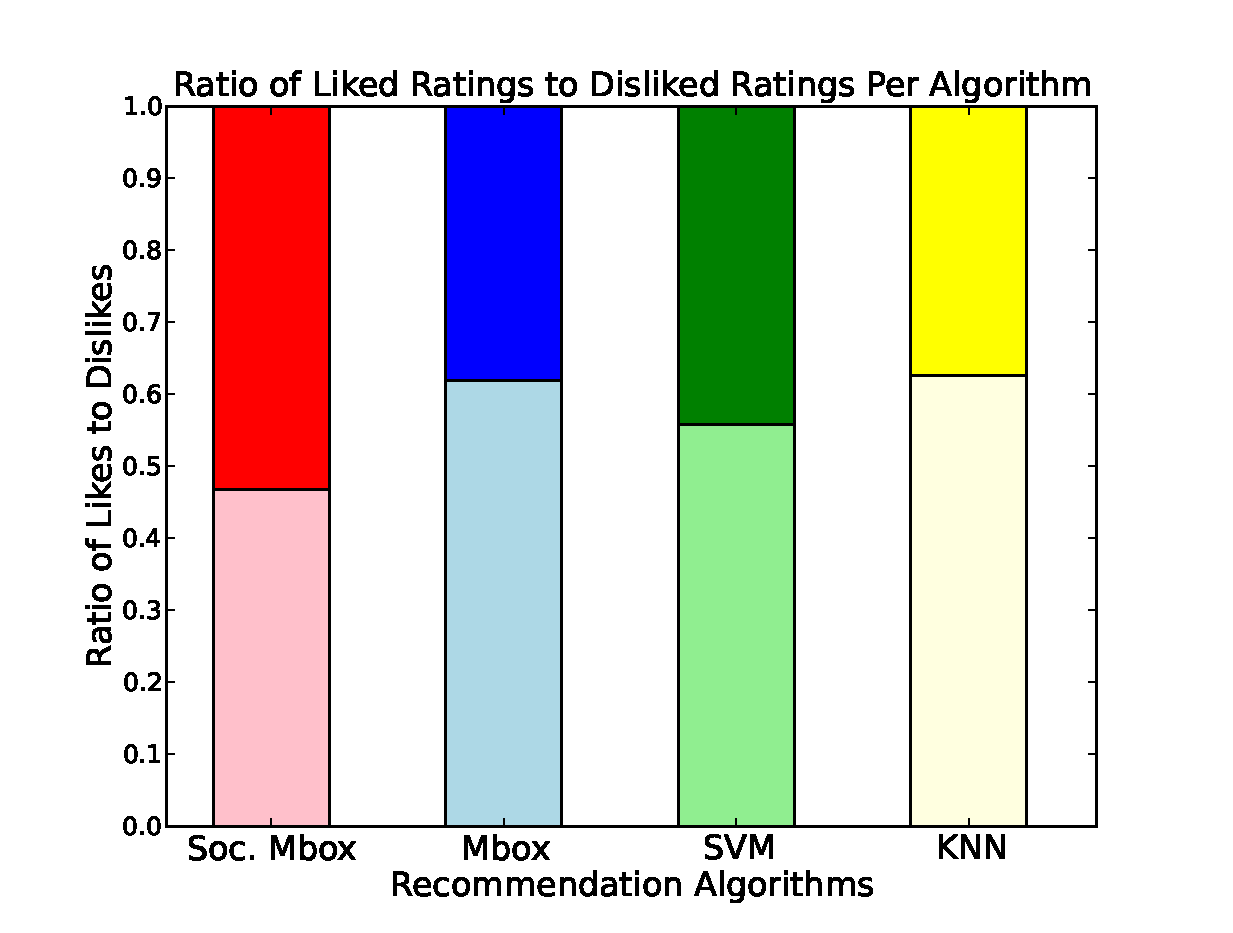
\includegraphics[scale=0.28]{img/live-likes1.eps}}
\subfigure{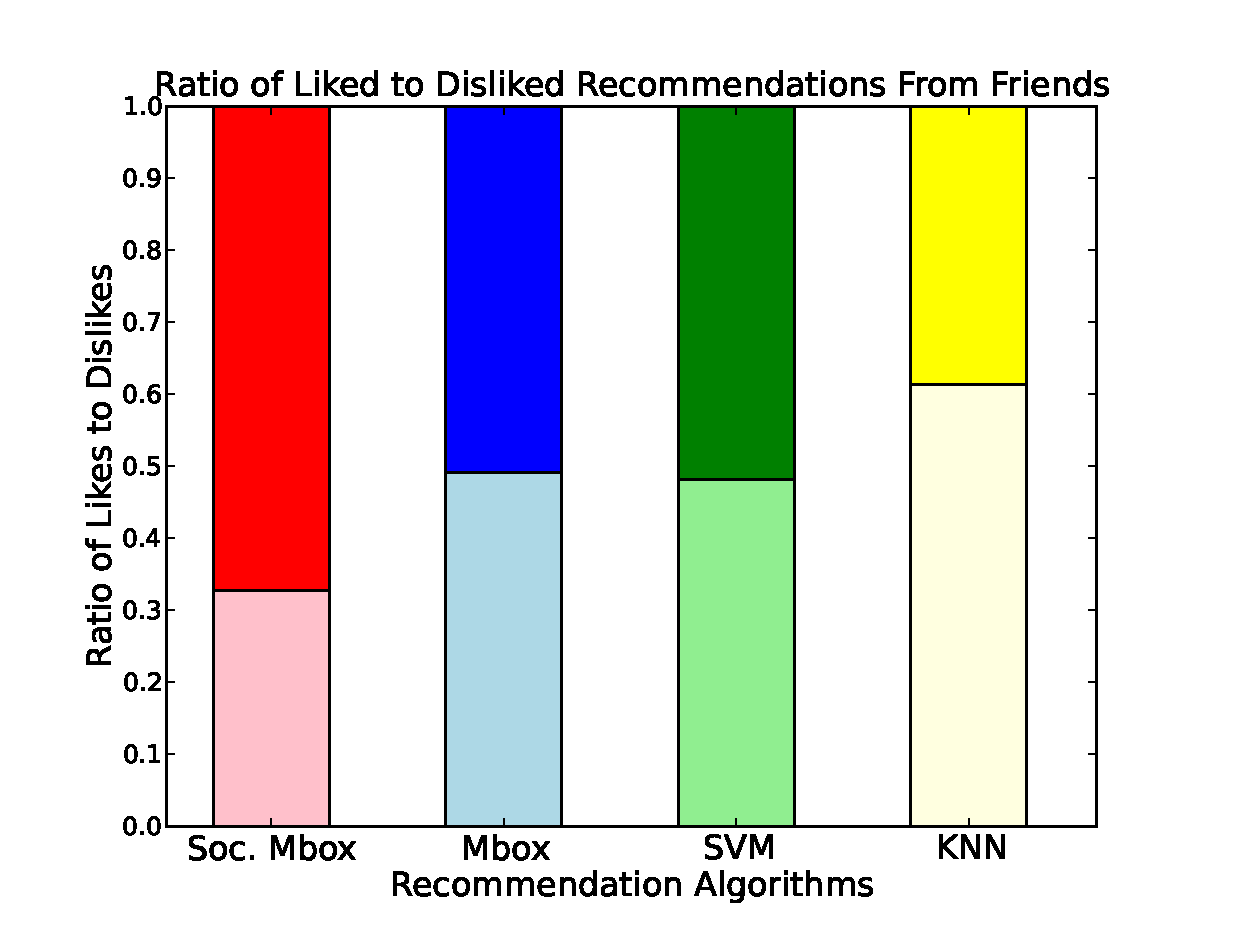
\includegraphics[scale=0.28]{img/live-friend-likes1.eps}}
\subfigure{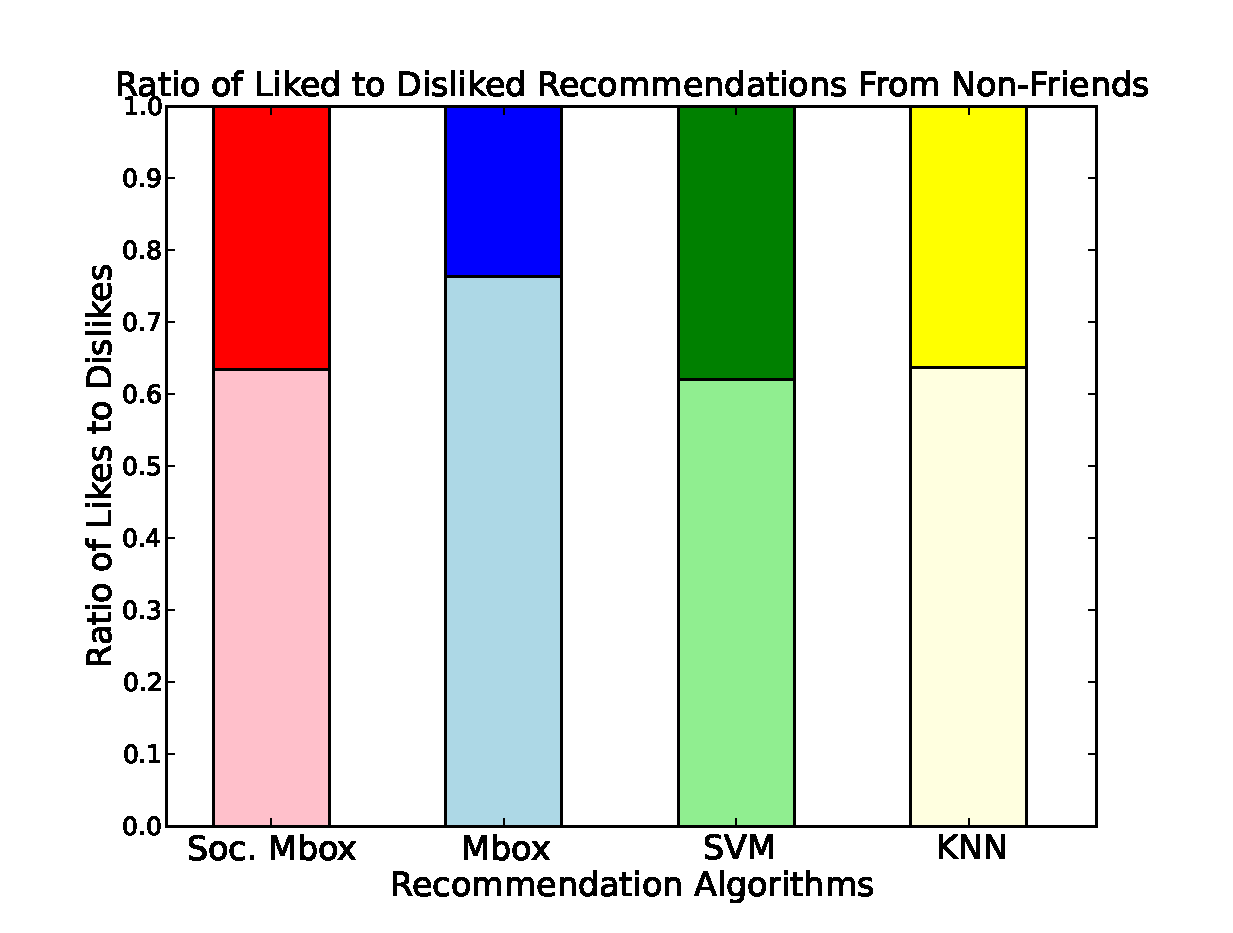
\includegraphics[scale=0.28]{img/live-nonfriend-likes1.eps}}
%\subfigure{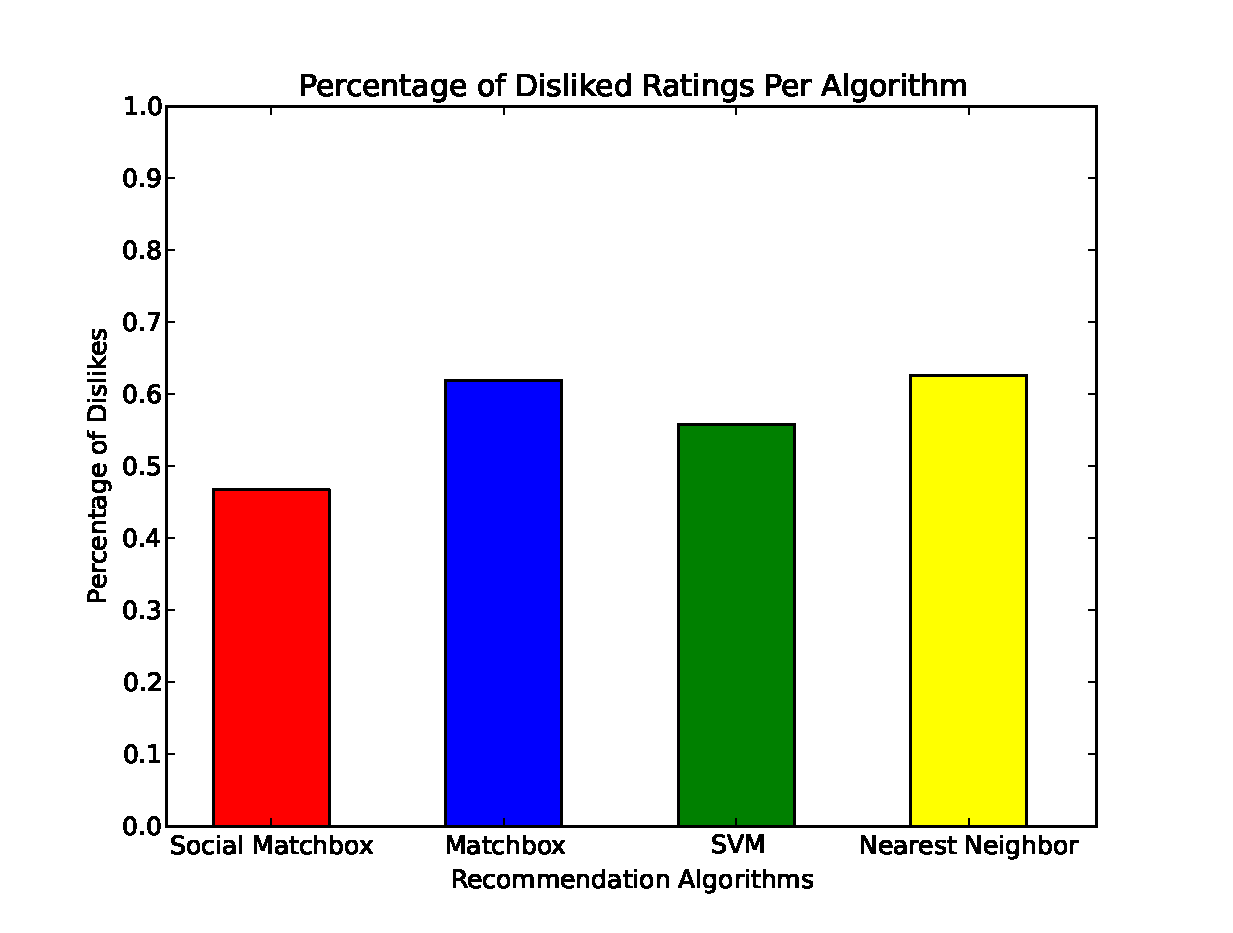
\includegraphics[scale=0.35]{img/live-dislikes1.eps}}
\caption{Results of the online live trials. The percentage of Liked
ratings are stacked on top of the percentage of Disliked ratings per
algorithm. Social Matchbox was found to be the best performing of the
four algorithms evaluated in the first trial.  *** Results of the online
live trials, split between friends and non-friends. The percentage of
Liked ratings are stacked on top of the percentage of Disliked ratings
per algorithm. There is a significant drop in performance between
recommending friend links and recommending non-friend links.}
\label{fig:OnlineResult1}
\end{figure*}

We also look at the algorithms with the results split between friend
links and non-friend links recommendations. Again, the results shown
in Figure~\ref{fig:OnlineFriend1} are the percentage of Like ratings
and the percentage of Dislike ratings per algorithm stacked on top of
each other with the Like ratings on top. As shown in
Figure~\ref{fig:OnlineFriend1}, all four algorithms experienced a
significant performance drop in the ratio of Likes to Dislikes when it
came to recommending non-friend links. This suggests that aside from
Liking or Disliking a link solely from the quality of the link being
recommended, users are also more likely to Like a link simply because
a friend had posted it and more likely to Dislike it because it was
posted by a stranger.

\subsection{Survey Results}

Near the end of the first trial, the LinkR users were invited to answer a survey regarding their experiences with the recommendations they were getting. They were asked a number of questions, with the following pertaining to the quality of the recommendations:

\begin{itemize}
\item{Do you find that ANU LinkR recommends interesting links that you may not have otherwise seen?}
\item{Do you feel that ANU LinkR has adapted to your preferences since you first started using it?}
\item{How relevant are the daily recommended links?}
\item{Overall, how satisfied are you with LinkR?}
\end{itemize}

They gave their answers to each question as an integer rating with range $[1-5]$, with a higher value being better. Results are shown in Figure~\ref{fig:survey1}. Their answers were grouped together according to the recommendation algorithm that was assigned to them, and the averages per algorithm are below.

As shown in Figure~\ref{fig:survey1}, Social Matchbox achieved higher survey scores than the other recommendation algorithms, in all four questions. The results of the survey reflected the results in the online live trial and confirms that Social Matchbox was the best recommendation algorithm in the first trial.
 
\begin{figure*}[t!]
\centering
\subfigure{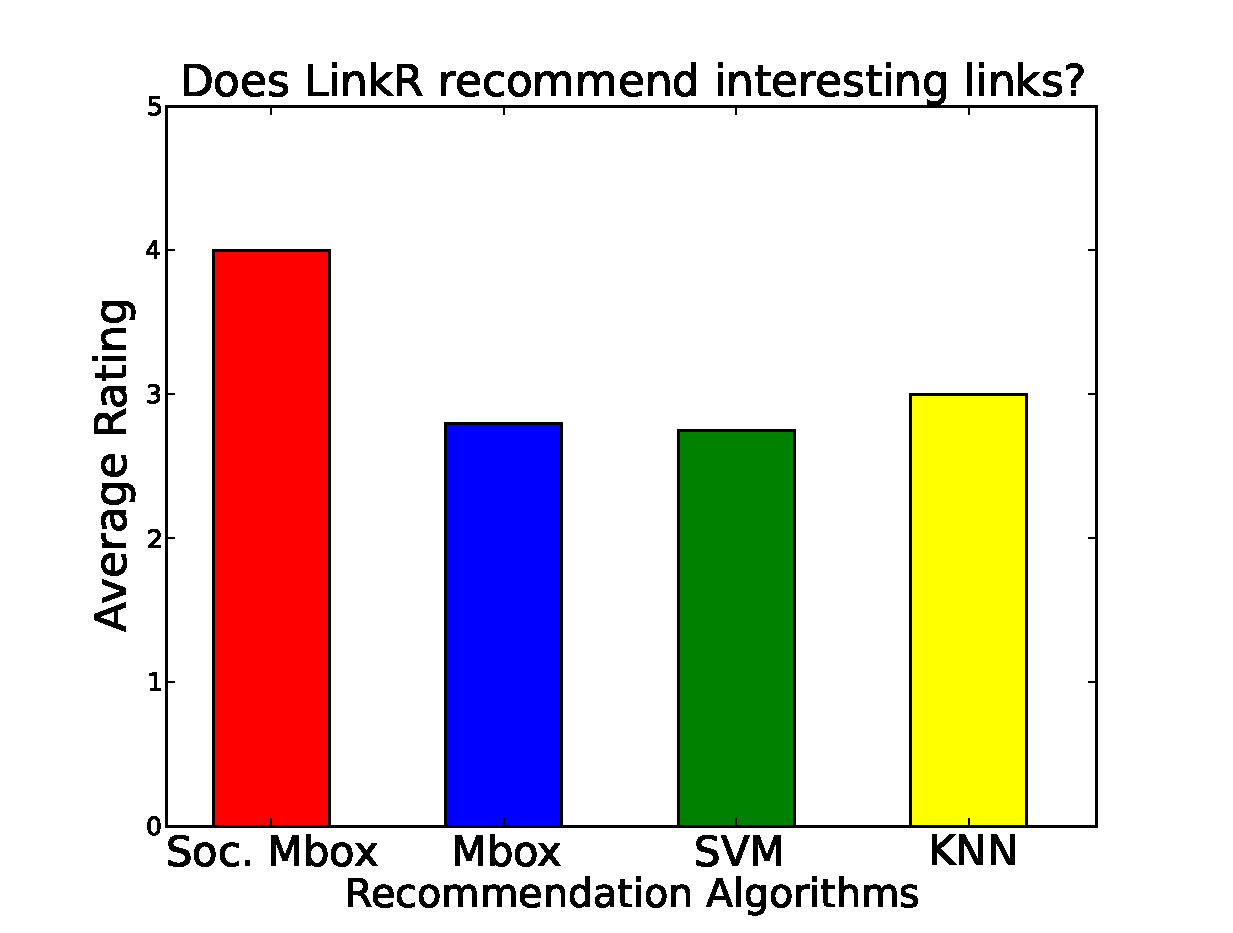
\includegraphics[scale=0.23]{img/not-seen.eps}}
\hspace{-6mm} \subfigure{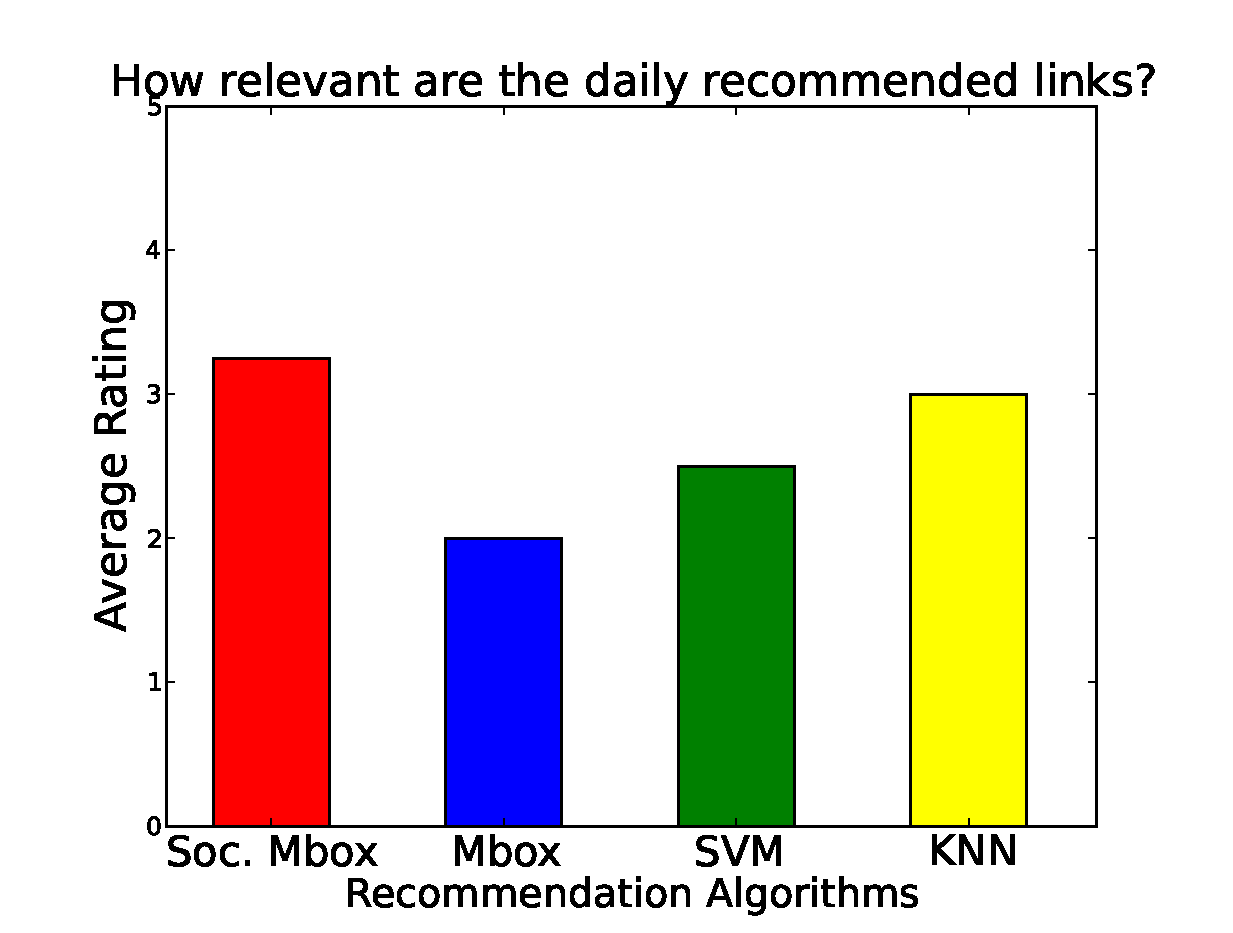
\includegraphics[scale=0.23]{img/relevant.eps}}
\hspace{-6mm} \subfigure{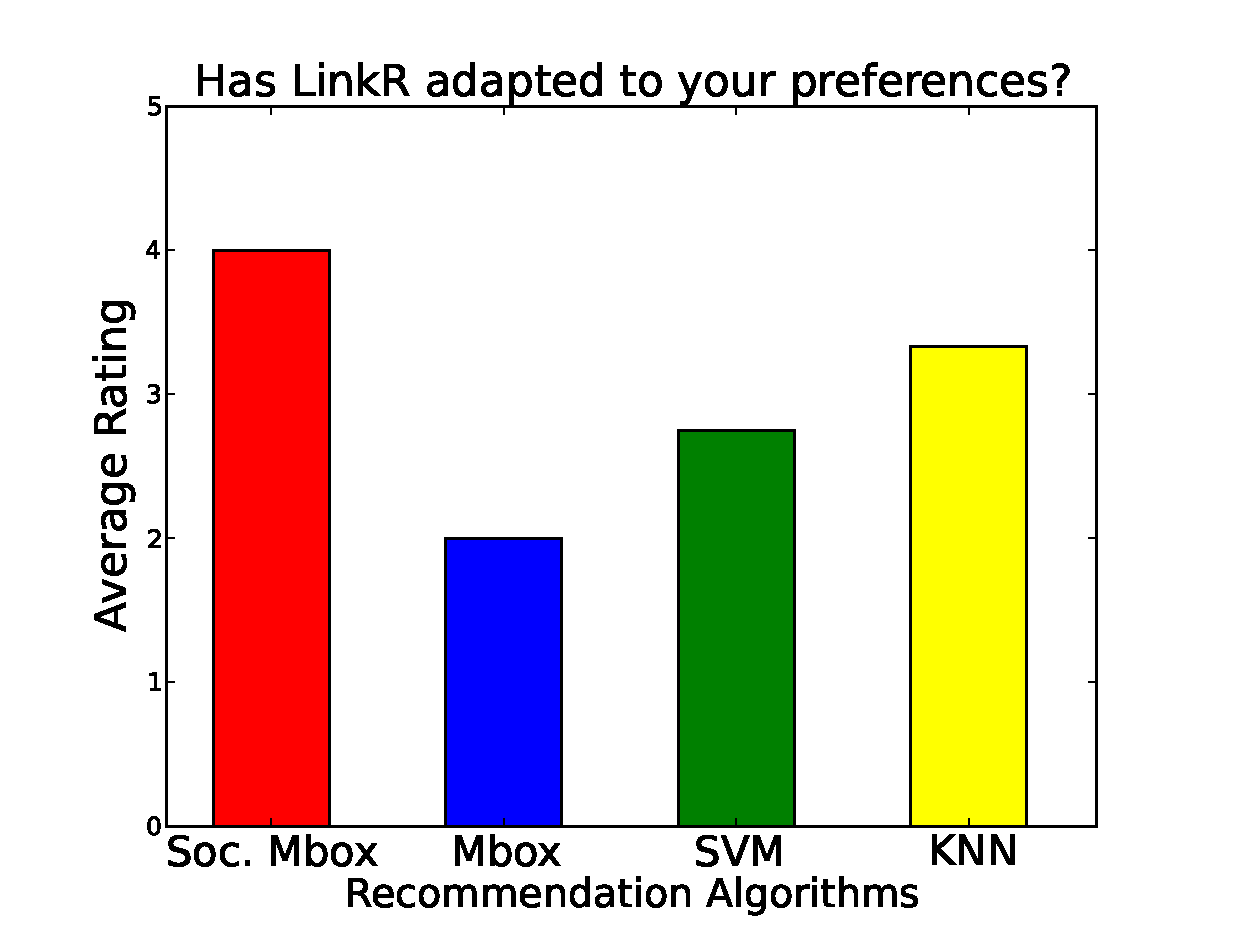
\includegraphics[scale=0.23]{img/adapted.eps}}
\hspace{-6mm} \subfigure{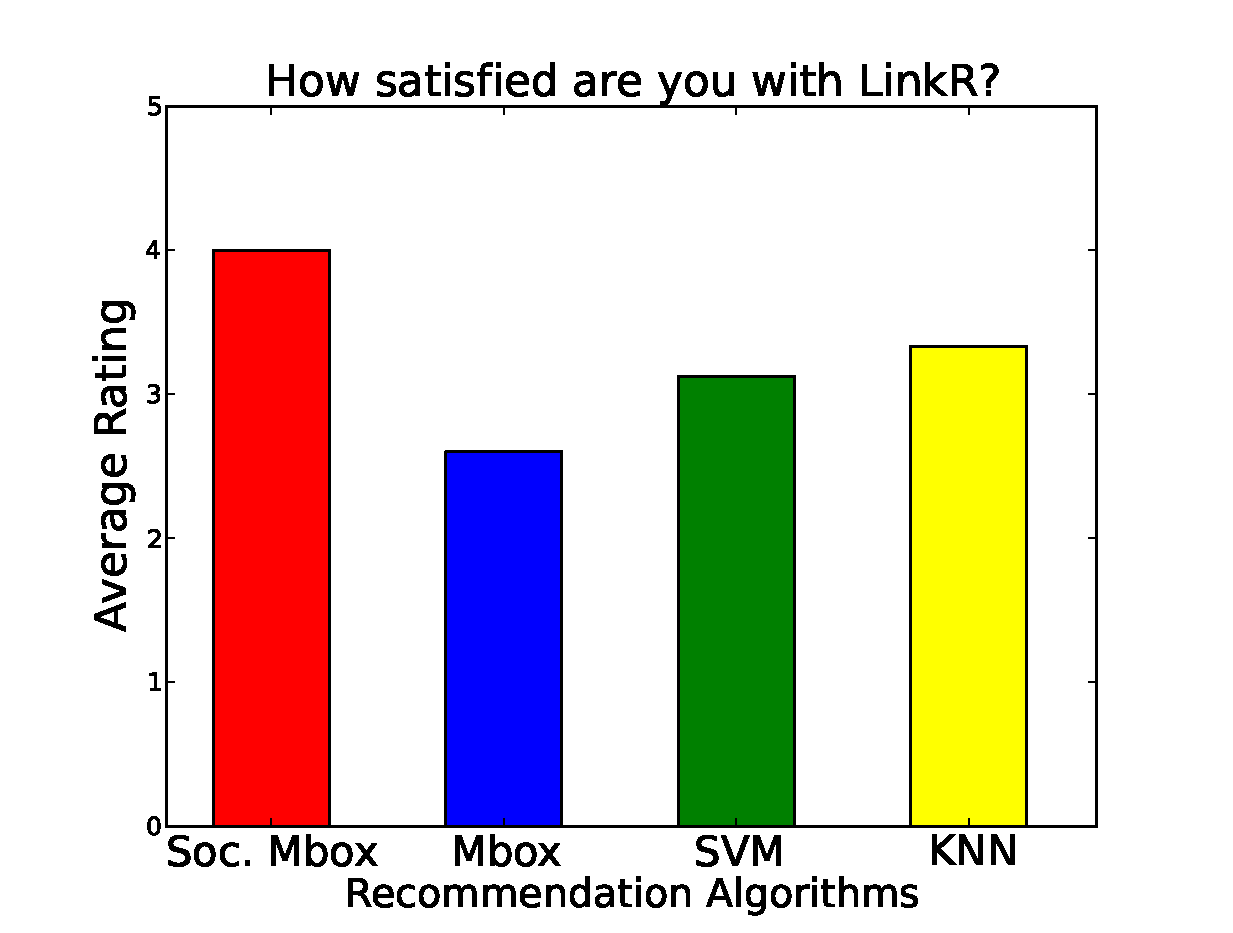
\includegraphics[scale=0.23]{img/satisfied.eps}}
\caption{Results of the user survey after the first trial. The survey answers from the users reflect the online results that Social Matchbox was the best recommendation algorithm in this trial.}
\label{fig:survey1}
\end{figure*}

\subsection{Summary}
At the end of the first trial, we have observed the following:

\begin{itemize}
\item{Social Matchbox was the best performing algorithm in the live user trial in terms of percentage of likes.}

\item{Social Matchbox received the highest user evaluation scores in the user survey at the end of the user trial.}

\item{Of the various combinations of training and testing data in the offline passive experiment, we found that training on the UNION subset and testing on the APP-USER-ACTIVE-ALL subset best correlated with the results of the live user trial and the user survey. Training on the UNION dataset had advantages compared to training on the other data subsets, namely that it had the large amount of information of the PASSIVE data and the explicit dislikes information of the ACTIVE data.}

\begin{comment}
Explain which offline evaluation correlates with both of these user feedback metrics... can you briefly explain why?  E.g., training on UNION gives you explicit negatives, which are crucial (side note, perhaps not for thesis: except maybe for NN which actually does need negatives!), and ranking evaluation really requires an accurate list of likes/dislikes for an accurate ranking metric which can only be had with the active data}
\end{comment}

\end{itemize}

In the next chapter, we discuss new techniques for incorporating social information and show how they improve on Social Matchbox.
